\documentclass[a4paper,10pt,twocolumn]{article}
\usepackage{lmodern}
\usepackage[english]{babel}
\usepackage[T1]{fontenc}
\usepackage[utf8]{inputenc}
\usepackage{graphicx}
\usepackage{float}
\usepackage[top=1cm,bottom=2cm,left=1cm,right=1cm]{geometry}
\usepackage{amsmath}
\usepackage{amssymb}

\title{Similarity of Mass Spectra}
\date{\today}
\author{Ondřej Podsztavek, podszond@fit.cvut.cz}

\begin{document}

\maketitle

\section{Project Description}

The goal of this project is to create an application which searches
in database of protein sequences for peptide sequences similar to input
mass spectra.

\subsection{Input}

Application inputs are mass spectra and database of protein
sequences.

\subsection{Output}

Output it set of peptide sequences similar to input mass
spectra sorted according to similarity.

\section{Solution Method}

To measure similarity, feature vectors from feature space \(\mathbb{U}\)
and similarity measure \(\delta: \mathbb{U} \times \mathbb{U} \to \mathbb{R}\)
are needed.

Each mass spectrum is set of a peptide fragments intensities. In order to create
feature vector, easy feature extraction method is applied. Mass spectrum
intensities are binned to equal-width bins.

Protein sequences are split into peptides according to rule that the
sequence is split after occurrence of amino acid 'K' or 'R' if it is not
followed by amino acid 'P'. Modified peptides from split peptides are
ignored and that mass spectrum for them is calculated based on b-ions with
charge 1. Intensities corresponding to obtained mass spectra are set to 1.
For more information please refer to~\cite{novak2009}.

Cosine similarity is chosen as similarity function. It computes the
L2-normalized dot product of vectors. That is, if \(x\) and \(y\) are vectors,
their cosine similarity \(\text{SIM}_{\cos}\) is defined as:

\[ \text{SIM}_{\cos}(x, y) = \frac{x^Ty}{\|x\|\|y\|} \]

\section{Implementation}

The application is divided into 4 modules:

\begin{itemize}
    \item mass spectra database operations,
    \item mass spectra preprocessing
    \item similarity measure,
    \item web application.
\end{itemize}

Programming language used is Python~3.6. From libraries the application requires
scikit-learn~0.19.1~\cite{scikit-learn}, NumPy~1.13.3,
SciPy~1.0.0~\cite{scipy}, Flask~0.12.2 and
pyteomics~3.4.2~\cite{Goloborodko2013}. Web application database is MongoDB 
and visualization are created be Vega-Lite library.

\subsection{Database Module}

The database module contains functions for working with database of
proteins sequences. The main two function are for database generation and
database load.

Database is generated from FASTA file format and stored as NumPy's NpzFile.
The NpzFile contains 3 NumPy matrices. First is the array of peptides.
Second is the array of \(\frac{m}{z}\) values. Last is the matrix of binned
mass spectra in which each row is a binned mass spectrum. This last
matrix is in LIL format.

The LIL (list of lists) sparse matrix stores one list per row with entries
containing the column index and the value. It is good format for incremental
construction.

\subsection{Similarity Module}

The similarity measure module contains the \(k\) nearest neighbor query 
(\(k\)NN). The query return matrix of indexes to database of size
\(n \times k\) where \(n\) is the number of mass spectra queried.
Row \(i\) contains indexes to most similar spectra in database in
descending order.

Cosine similarity is computed using function \texttt{cosine\_similarity}
from scikit-learn library. Its inputs are two LIL sparse matrices and output
is CSR sparse matrix. Sparse matrices are used because the feature vector
contains a lot of zero value and are difficult to store in memory.

\subsection{Preprocessing Module}

The spectra preprocessing module contains function for mass spectra
handling and generation.

Function \texttt{read\_mgf} uses
\texttt{pyteomics.mgf.read} to parse MGF format file because that it the
only format this application supports.

\texttt{compute\_mass\_spectrum} function serves to
compute mass given a peptide sequence.
Database generation procedure calls this function mainly.
It calls \texttt{pyteomics.mass.calculate\_mass} which return the intensity.

Last interesting function is the feature extraction method implemented as
\texttt{bin\_spectrum} function which calls
\texttt{scipy.stats.binned\_statistic} to bin a spectrum.

\subsection{Web Application}

The web application is built on Flask framework. There is 5 different
views.

Usual workflow is to upload MGF file on the index page with
selected \(k\). The user is them redirected to result view where it is
possible to go to each spectrum for the MGF file and see which similarities
were found.

Moreover, views with database statistics and past results are provided. 

\section{Output Example}

Figure~\ref{fig:sample} shows an example result page for a spectrum with 
one similar spectrum found.

\begin{figure}[H]
    \begin{center}
        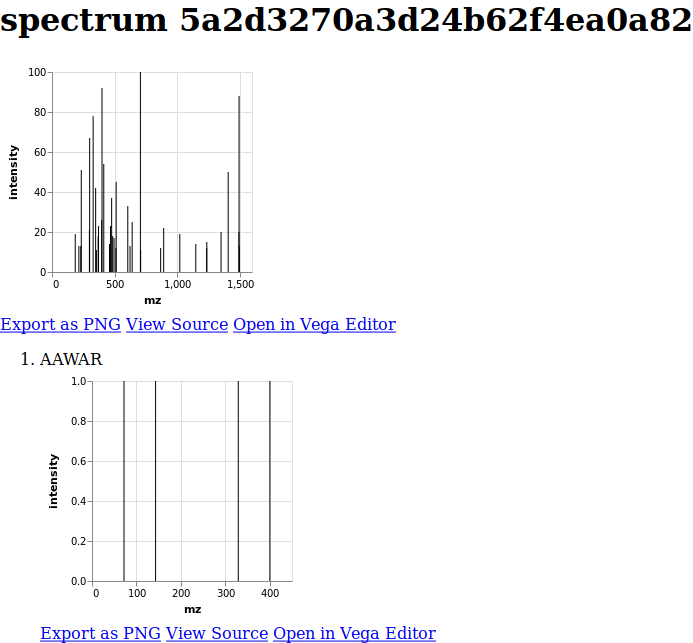
\includegraphics[width=6cm]{img/output-sample}
    \end{center}
    \caption{Flask application result page example.}
    \label{fig:sample}
\end{figure}

\section{Experiments}

This section presents some experiments with speed and accuracy of
implemented application.

Table \ref{table:experiments} show statistics of \(k\)NN query.
Testing data are a protein database of 218513 peptide sequences and a MGF file
with 1569 labeled mass spectra. Result for 3 different bin sizes are presented.
Accuracy if the spectrum was between top 1, 5 or 10 found peptides sequences.
CPU times for the different times are also shown.

\begin{table}[H]
    \begin{center}
        \label{table:experiments}
        \begin{tabular}{l|rrr}
            & \multicolumn{3}{c}{\textbf{bin size}} \\
            \textbf{accuracy measure} & 0.1 & 0.5 & 1 \\
            \hline
            top 1 (\%) & 6.12 & 6.37 & 6.50 \\
            top 5 (\%) & 7.46 & 8.09 & 8.22 \\
            top 10 (\%) & 8.29 & 8.80 & 8.86 \\
            CPU time (s) & 20.1 & 24.7 & 24.0 \\
        \end{tabular}
        \caption{
            Accuracy of similarity search in percents for different bin sizes.
            Top 10 accuracy measures if the searched peptide sequence is between
            the first 10 returned results. Accordingly are defined the top 5
            and top 1 accuracy. The last row show CPU time needed to compute
            the cosine similarity.
        }
    \end{center}
\end{table}

Results show the problem addressed in this project is hard. Accuracy of 8.29\%
for the target peptide to appear in top 10 found peptides is bad and there
should deployed some preprocessing procedures to improve the result.
Some approaches are also suggested in the next section.

From time perspective the database generation takes approximately 9 and half
minutes. But the database is generated once and then use so it is no concern.
Then, each query takes approximately 20.1--24.7 seconds. Because this application
is not based on fast user interation it is also fine.

\section{Discussion}

This project tries to solve hard problem of similarity search in mass spectra.
Cosine similarity method was implemented and tested for 3 different bin sizes.
The results are not satisfactory but prove that this concept works.

To further improve the accuracy there is a lot of extension that can be added to
this application. For example y-ions and a-ions might be added to database
and user might be offered the choose to compare to these spectra. Also the mass
spectra can be computed for different charges. Lastly peptide modifications are
not taken into account.

From application perspective range query could be implemented but it will not
improve search accuracy.

\section{Conclusion}

This project's goal was to implement application for similarity search in
database of protein sequences for peptides according to its mass spectrum.
Experiments section presents unsatisfactory results but generally the problem
of searching for similar peptides from mass spectra is hard due to noise and
imperfection during mass spectra retrieval.

\bibliography{report}{}
\bibliographystyle{plain}

\end{document}
